\chapter{Mattock: A modernized Open Computer Forensics Architecture}
This appendic tries to show the big picture of a prospect computer forensics framework that builds on both the good parts of the Open Computer Forensics Architecture (OCFA), and the concepts and sub-systems introduced in the research paper. The idea of this appendix is to sketch a  the rough outlines of a possible OCFA inspired framework using modern day information technology components and insights gained from years of OCFA usage and the analysis done in Apendix-A. A framework that could fill the gap left by the discontinuation of OCFA development by the dutch police. While this gap has been filled successfully for dutch law enforcement by the non-open Xiraf framework developed by the Netherlands Forensic Institute, and while on a smaller scale the frameworks provided by PyFlag and the Sleuthkit Framework non of the open source solutions have yet attempted to leverage either modern technologies with the potential to seriously reduce scalability bottlenecks on multi-node setups or to address the significant performance issues with potentially unnesisary disk-IO. Neither have the two frameworks managed to provide the accademic community with a framework suitable for serious computer forensic research projects of the scale of for example the FIVES project that used OCFA at its core. While implementation of a full framework with the required properties fals far outside of the scope of a single MsC research project, this chapter will provide the architectural outline of such a framework and will explain how MatockFS would play a pivitol role in the realization of such a framework. We shall address the prospect Framework as Mattock. The idea of the naming stems from the naming of the carving tool scalpel. The idea is that while a tool the size of and with the precission of a scalpel is indispensible at any scale, if you want to scale up your investigations to the scale of an archeological dig, you will need bigger tools like a mattock. Well, its just a working name. Anyone picking up on this paper is invited to come up with a more suitable name for the resulting framework. 
\section{The OCFA architecture}
\begin{figure}
\centering
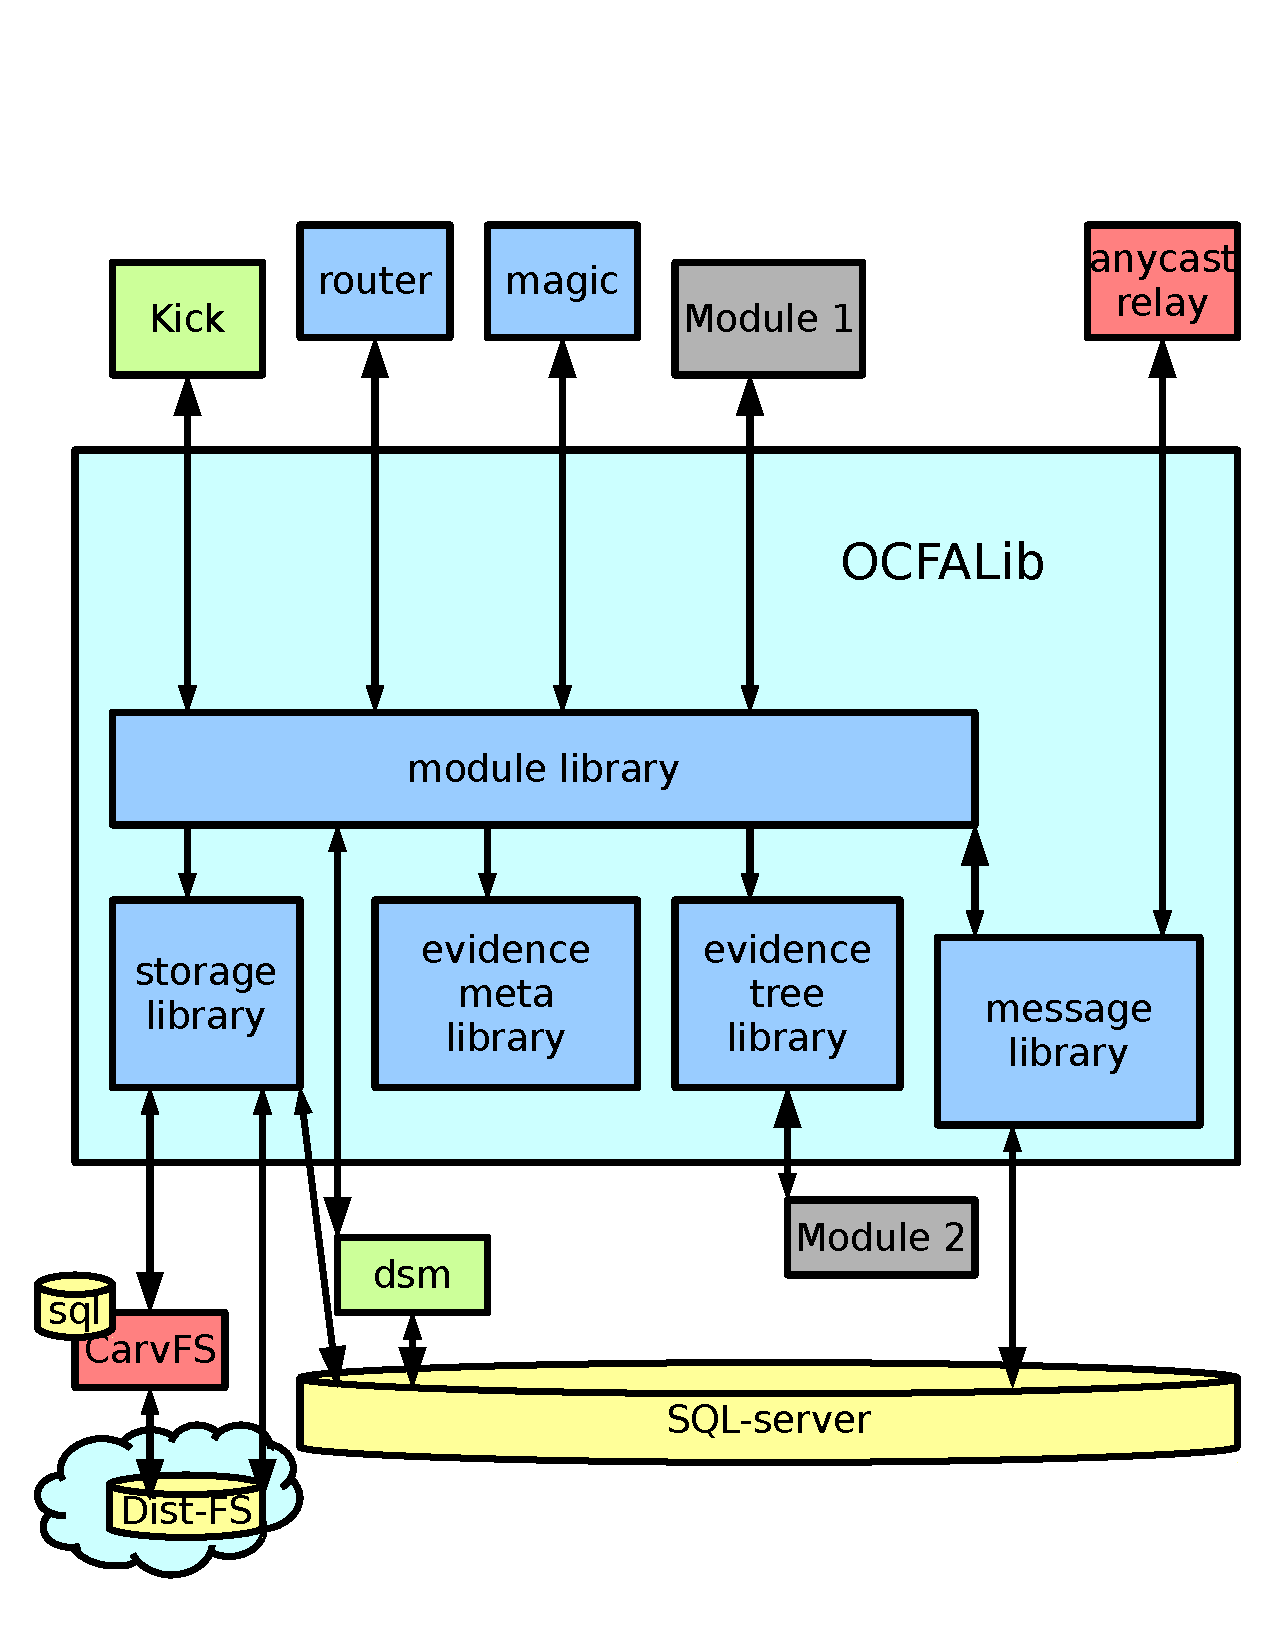
\includegraphics[width=100mm]{mattock/libraryview.pdf}
\caption{The base OCFA architecture}
\label{fig:FlowInOut}
\end{figure}
If we look at the OCFA architecture, at the core we basically see a fully custom build asynchonous messaging framework for processing modules that communicate with a small set of netwotking components that act to combine the modules into dynamic chains of tools that are applied to parts of the forensic evidence data. The use of comodity software components is mostly limited to the pervasive use of XML technology and a central relational database. We shall have a look at some of the core components of the OCFA framework.
\subsection{The AnyCast Relay and Persistent Priority Queue}
At its basis, OCFA was a message passing concurency based system. One known issue with message passing concurency is the use of buffers. While message passing envinronemts like the Erlang programming language and platform opt to put producing processes to sleep when buffers fill up, OCFA opted for a different approach. In OCFA, the message passing buffers were managed by on-disk persistent priority queues. As these queues only contained referenced to in database large text objects, the persistent queues were meant and designed to be fully crash resistent. The priority queus had a special 'never' priority to hold messages that were observed to crash specific modules. This allowed modules to be restarted and to skip problematic data untill a maintenance programmer would look at the problematic data and buggy module to fix the problem and re-submit the messages in the never queue for further processing. The Anycast relay was built on top of the persistent priority queue. Every module connected to the Anycast relay and registered as a consumer of a certain type (a module instance) and would go into a message processing event loop asking the Anycast relay for new jobs. When a module was done with a peice of evidence data, or when a module derived a sub entity from such data (for example an attachment as child entity of an e-mail message), the module would send a message to the Anycast Relay adressed at a special process named the router. The AnyCast would keep track of irresponsive and broken network connections and would play an important role in having stale or crashed modules restarted in a way not unlike what is common practice in Erlang based architectures. On such a detected crash, messages that were still pending a respnse would be put aside in the never queue to be looked at by a technision at a later point in time. In OCFA the AnyCast relay served as a single server for all modules, independent of the server these modules would run on.
\subsection{OcfaLib, a domain specific asynchonous framework}
While today NodeJS has mainstreamed the idea of a generic asynchonous framework, and while in other programming languages generic asynchonous frameworks such as Twisted for Python or Boost::asio for C++ have been available for quite a while, OCFA was first built long before such systems became mainstream. As a result, OCFA basically ended up building its own asynchonic processing framework. We could say that OcfaLib, the C++ OCFA library was a domain specific asynchonous framework for use with the AnyCast server. 
\subsection{The lagacy Module API}
OCFA came with two quite distinct module Application Programming Interfaces (APIs). This fact was the result of chronology of development. The first version of OCFA came with a module API not much unlike that of the current day sleuthkit framework. A module would get a file to process and could add meta data to that file, or, when it wanted to for example mark an extracted e-mail attachment as child entity, would submit that to the framework. The API consisted of a module initialisation part and a single method called 'processEvidence' that a module was supposed to overload. From within ProcessEvidence the module could either add meta or submit a child entity with added meta date.
\subsection{The Treegraph API}
After new modules got added to OCFA, the legacy module API was found to be lacking in the meta-data area. The problem was that a module deriving a tree of children would not be able to set meta-data for deeper child entities. Only level zero and level one meta data was possible. As a result, the more powerfull treegraph API was added. As porting old modules to the new API was considered a waste of precious development time, the old API was also still continued after the introduction of the new API.
\subsection{The legacy CAS storage}
\subsection{CarvFS}
\subsection{The meta-data based message router}
\subsection{The use of an SQL server}
\section{PyFlag}
\section{The Sleuthkit framework}
\section{Non-open frameworks}
\section{New insights}
\section{A modernized OCFA inspired open-source architecture}
\begin{figure}
\centering
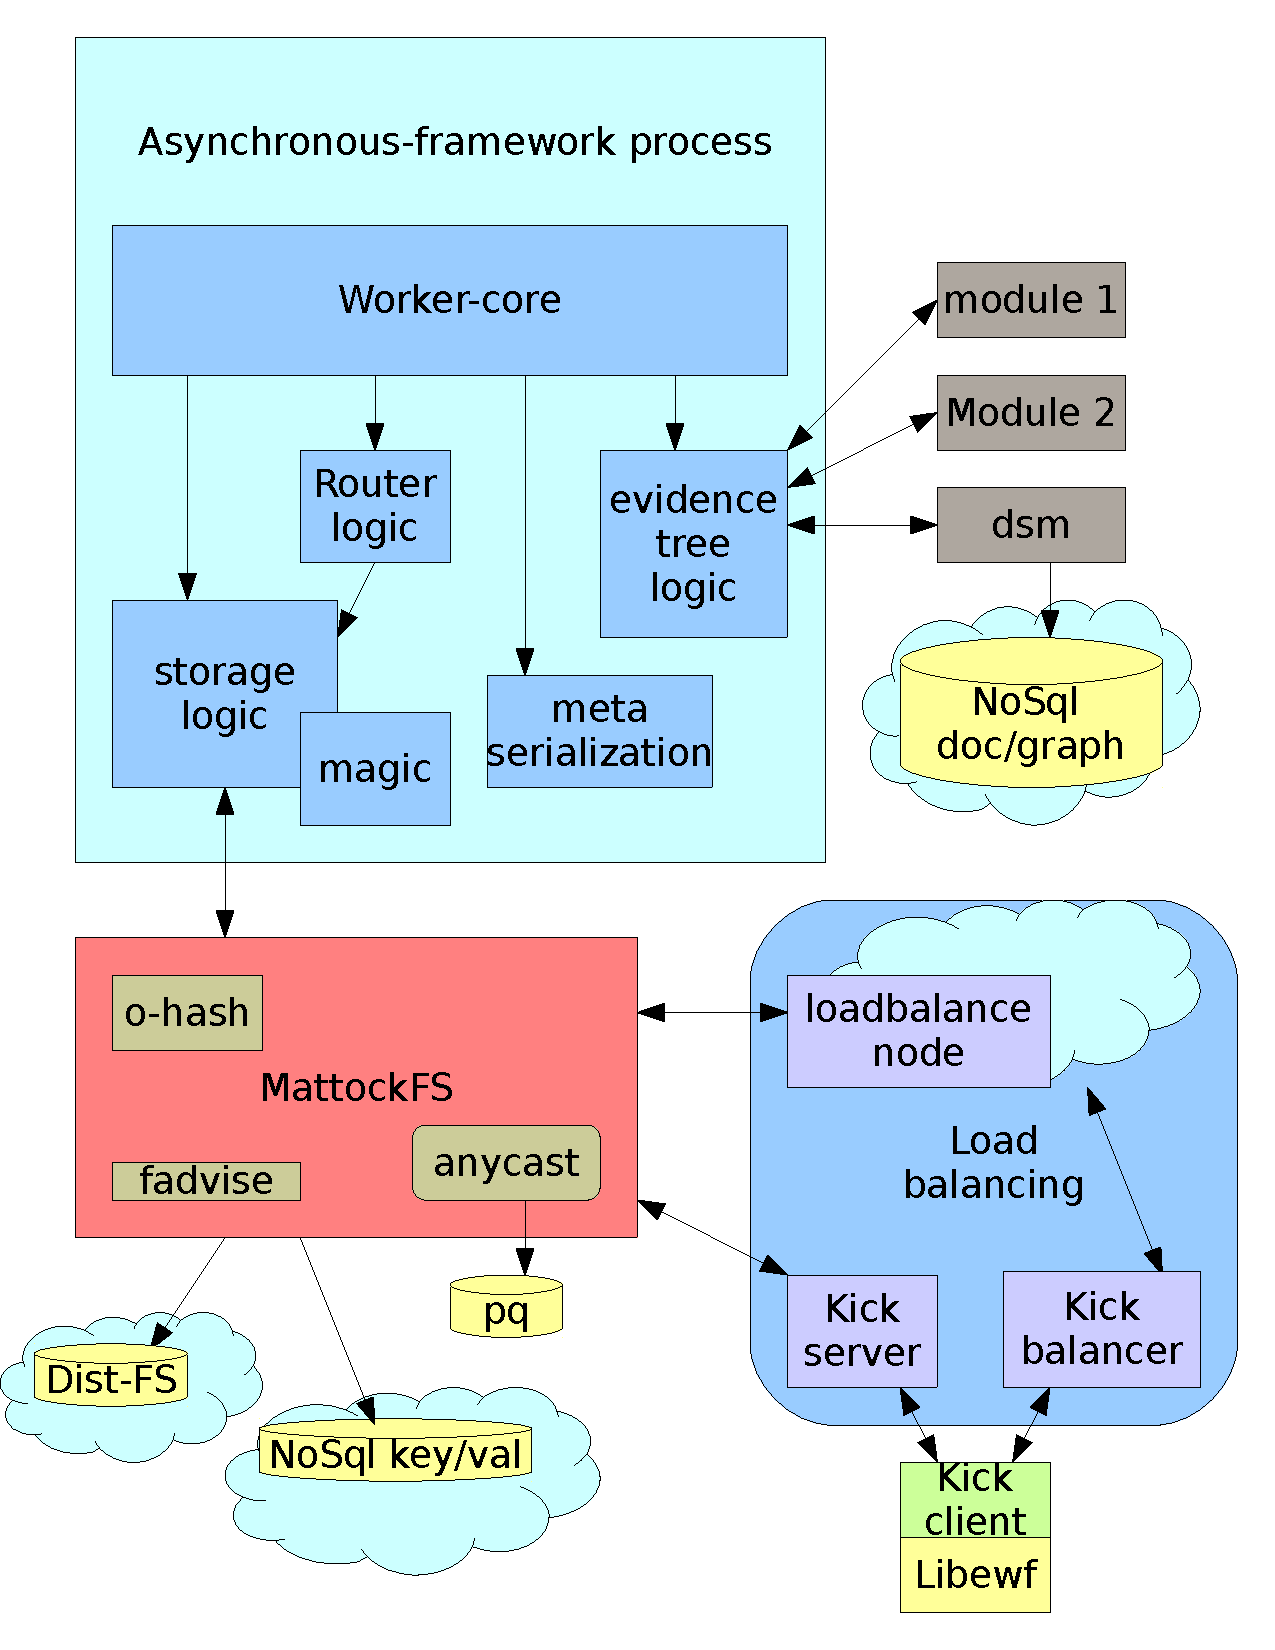
\includegraphics[width=100mm]{mattock/libraryviewmattock.pdf}
\caption{The base Mattock architecture}
\label{fig:FlowInOut}
\end{figure}
\subsection{MattockFS \& the distributed longpath store}
\subsection{The AnyCast Monitor meshup}
\subsection{Client/Server kickstarting}
\subsection{Effective distributed system usage}
\subsection{Store-system embedded libmagic functionality}
\subsection{Distributed routing logic}
\subsection{From SQL to Document/Graph based NoSQL}
\subsection{Using language-native asynchonous frameworks}
\subsection{A single tree-graph, lambda and asynchonous operation oriented API}
\subsection{Conclusion}
